\chapter{Experiments}
\label{chapter:experiments}

This chapter

\begin{itemize}
    \item describes the experiments in terms of reproducible steps, settings, parameters, conditions;
    \item presents and discusses results.
\end{itemize}

Ultimately the experiments aim to study transfer learning in the specific domain of skin lesion classification, as well as compare its efficacy against simpler and more traditional learning schemes, by training and testing several models of different architectures and drawing helpful conclusions about the use of transfer learning techniques.

\section{VGG16 Transfer Learning Experiments}

Based on the transfer learning techniques introduced in chapter \ref{chapter:sota}, models of the VGG16 architecture (again illustrated in figure \ref{fig:vgg16_reillustration}) pre-trained on ImageNet will be explored in order to repurpose the parameters to a new model for skin lesion classification and draw conclusions about its efficacy.

\begin{figure}[ht]
    \centering
    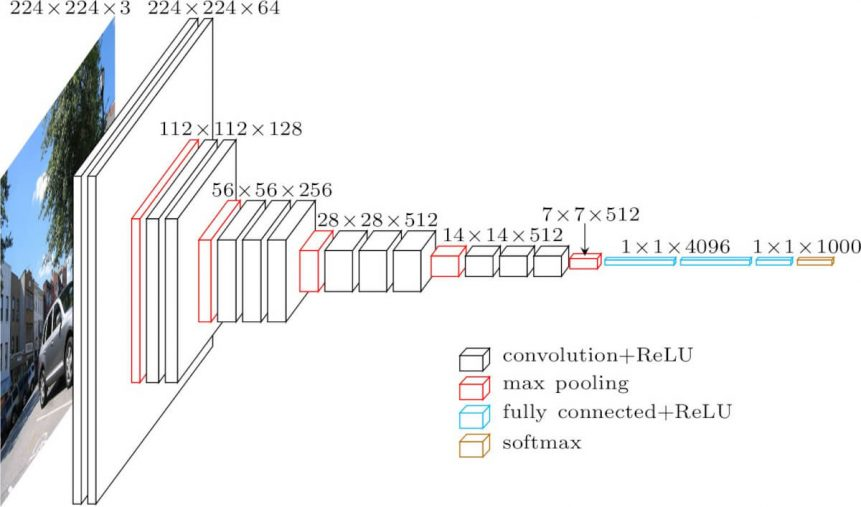
\includegraphics[width=1.0\textwidth]{figs/vgg16.jpg}
    \caption{Architecture of the VGG16 convolutional neural network \cite{vgg16}.}
    \label{fig:vgg16_reillustration}
\end{figure}

It is hypothesized that extracting parameters from lower layers of models trained for ImageNet classification can provide good performance, because the former presumably provide low-level features (e.g., shapes or lines) that are still useful for skin lesion classification whereas the latter provide very high-level concepts (e.g., dogs, cats) that are most relevant for classification in the ImageNet domain and otherwise needs fine-tuning to the target dataset.

In particular, the basic unit in the VGG16 network is the convolutional block, which is comprised by a stack of convolutional layers and one pooling layer. These convolutional blocks are then further stacked together to progressively build higher level feature maps at the end of each block. To verify this, one can run a sample input (figure \ref{fig:sample_input}) through the original VGG16 model pre-trained on ImageNet and visualize the activations at the end of each block (after its pooling layer).

\begin{figure}
    \centering
    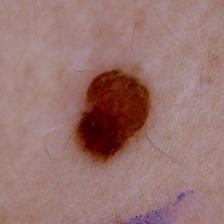
\includegraphics[width=0.4\textwidth]{figs/sample_input.jpg}
    \caption{A sample of the ISIC2018 train set showing a clear separation of background (skin) and foreground (lesion).}
    \label{fig:sample_input}
\end{figure}

As expected, the features detected in the early layers of the network (figure \ref{fig:vgg16_block1}) activate for low level concepts like shapes (the border around the lesion), background (the skin), and foreground (the lesion itself).

\begin{figure}
    \centering
    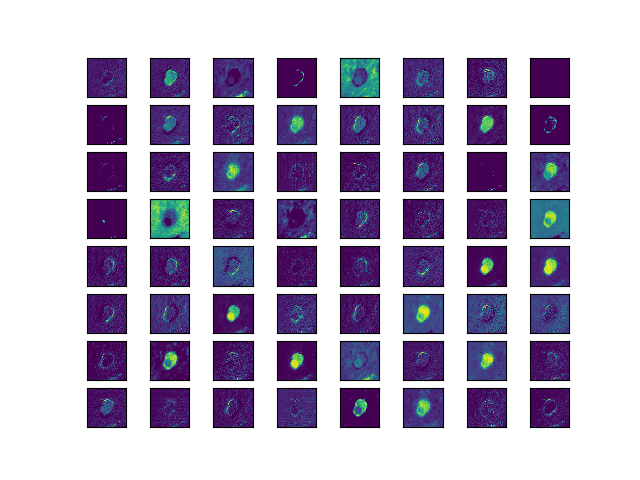
\includegraphics[width=1.0\textwidth]{figs/vgg16_block1.png}
    \caption{The 64 feature maps at the pooling layer of block 1 of the VGG16 model exactly as trained on ImageNet.}
    \label{fig:vgg16_block1}
\end{figure}

Then features in the middle layers (block 3 in figure \ref{fig:vgg16_block3}) are progressively more abstract.

\begin{figure}
    \centering
    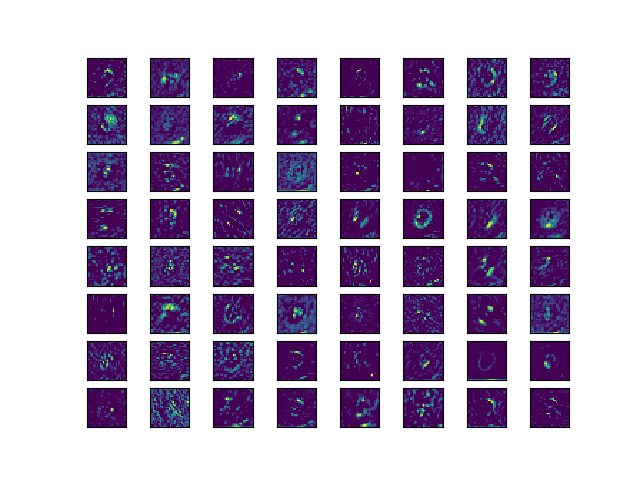
\includegraphics[width=1.0\textwidth]{figs/vgg16_block3.png}
    \caption{64 of the 256 feature maps at the pooling layer of block 3 of the VGG16 model exactly as trained on ImageNet.}
    \label{fig:vgg16_block3}
\end{figure}

Finally at the last block of the network the feature maps exhibit much higher level (and low dimensional) concepts (figure \ref{fig:vgg16_block5}) completely incomprehensible to the human eye.

\begin{figure}
    \centering
    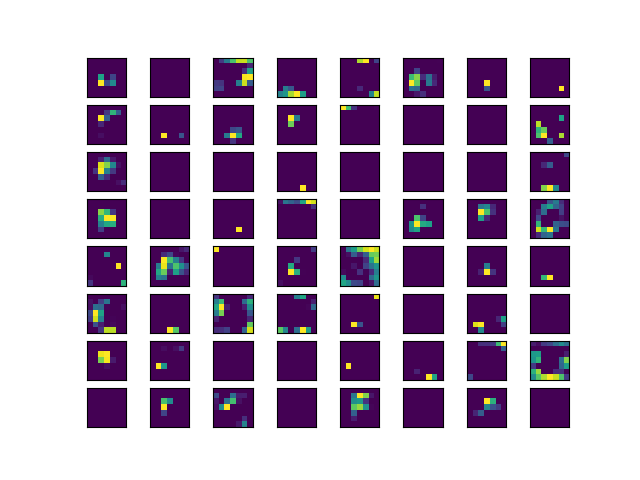
\includegraphics[width=1.0\textwidth]{figs/vgg16_block5.png}
    \caption{64 of the 512 feature maps at the pooling layer of block 5 of the VGG16 model exactly as trained on ImageNet.}
    \label{fig:vgg16_block5}
\end{figure}

Presumably, optimal transfer learning from the VGG16 pre-trained model is dependent on the layer up to which parameters are extracted from. Extracting all layers and perhaps even fine-tuning them to the target dataset is a sound strategy, but in some cases it might be useful to extract only a subset of the layers in order to produce a smaller model for applications where space (occupied by the model) and computation (required by the forward pass of an inherently deeper model) are at a premium (e.g. smartphones). Both of these cases (and more) will be explored.

The layers where this extraction and freezing of parameters occur can be seen as variables in order to later quantify the effectiveness of a particular strategy for extracting and freezing parameters:

\begin{itemize}
    \item the number of the layer $e$ up to which parameters will be extracted;
    \item the number of the layer $f$ up to which parameters will be frozen.
\end{itemize}

For narrative and reproducibility purposes, the variables $e$ and $f$ will refer to the index of the layers as implemented by \verb|tf.keras.applications.vgg16|\footnote{\url{https://www.tensorflow.org/api_docs/python/tf/keras/applications/VGG16}}. VGG16 is named after the 16 layers of parameters found in its 13 convolutional layers and 3 fully-connected layers, not to be confused with the total number of layers in the model as implemented by \verb|tf.keras.applications.vgg16| summarized below:

\begin{itemize}
    \item Layer 0 is the input layer (\verb|input_1|) and will not be considered as it merely represents the original input;
    \item Layers 1-3 constitute the first convolutional block (\verb|block1_conv1|, \verb|block1_conv2|, \verb|block1_pool|);
    \item Layers 4-6 constitute the second convolutional block (\verb|block2_conv1|, \verb|block2_conv2|, \verb|block2_pool|);
    \item Layers 7-10 constitute the third convolutional block (\verb|block3_conv1|, \verb|block3_conv2|, \verb|block3_conv3|, \verb|block3_pool|);
    \item Layers 11-14 constitute the fourth convolutional block (\verb|block4_conv1|, \verb|block4_conv2|, \verb|block4_conv3|, \verb|block4_pool|);
    \item Layers 15-18 constitute the fifth convolutional block (\verb|block5_conv1|, \verb|block5_conv2|, \verb|block5_conv3|, \verb|block5_pool|);
    \item Layers 19-22 constitute the classifier layers (\verb|flatten|, \verb|fc1|, \verb|fc2|, \verb|predictions|) and will not be considered.
\end{itemize}

In this work the pooling layers at the end of each of the five convolutional blocks will be considered for parameter extraction, i.e., $e$ will take values $e \in \{18, 14, 10, 6, 3\}$. Layers will be frozen accordingly, i.e., $f$ will take values $e \in \{18, 14, 10, 6, 3, 0\}$ such that $e \geq f$. For example:

\begin{itemize}
    \item $e = 18$ and $f = 14$ means that parameters are extracted up to layer 18 but the parameters up to layer 14 are frozen and will not be updated;
    \item $e = 14$ and $f = 6$ means that parameters are extracted up to layer 14 but the parameters up to layer 6 are frozen and will not be updated;
    \item $e = 10$ and $f = 0$ means that parameters are extracted up to layer 10 but no parameters will be frozen and thus will all be updated;
    \item $e = 10$ and $f = 14$ can not take place simultaneously since there is no meaning to extracting the first 10 layers and freezing the first 14 after having extracted only 10 of them.
\end{itemize}

The same examples are implemented in \verb|tf.keras| in code snippet \ref{code:vgg16}:

\begin{listing}[ht]
\begin{minted}{python}
def vgg16(e, f, l2):
    assert e >= f

    # Regularizer
    r = tf.keras.regularizers.l2(l2)

    # Extract and freeze pre-trained model layers
    vgg16 = tf.keras.applications.vgg16.VGG16(include_top=False)
    model = tf.keras.models.Sequential()
    for i in range(0, e+1):
        layer = vgg16.layers[i]
        layer.trainable = True if (i > f) and helpers.has_parameters(layer) else False
        layer.kernel_regularizer = r if helpers.has_parameters(layer) else None
        model.add(layer)

    # Classifier
    model.add(tf.keras.layers.GlobalAveragePooling2D())
    model.add(tf.keras.layers.Dense(units=512, activation='relu', kernel_regularizer=r))
    model.add(tf.keras.layers.Dense(units=1, activation='sigmoid', kernel_regularizer=r))
    return model

m1 = vgg16(18, 14, 0.0001)
m2 = vgg16(14, 6, 0.0001)
m3 = vgg16(10, 0, 0.0001)
\end{minted}
\caption{Function that extracts parameters from the VGG16 pre-trained model up to layer $e$ and freezes the parameters of the first $f$ layers, adds a global average pooling layer, adds a fully-connected layer of 512 ReLU-activated neurons, and adds a fully-connected layer of 1 sigmoid-activated neuron for binary classification.}
\label{code:vgg16}
\end{listing}

The following cases of transfer learning will be studied:

\begin{itemize}
    \item total parameter extraction ($e = 18$) without fine tuning ($f = e = 18$);
    \item partial parameter extraction ($e < 18$);
    \item total parameter extraction ($e = 18$) with fine tuning ($f < e$).
\end{itemize}

\subsection{Total Parameter Extraction without Fine Tuning}
\label{section:total_parameter_extraction_without_fine_tuning}

Arguably the simplest case is to extract and freeze all layers (i.e., $e = f = 18$), feed them to a classifier, and effectively only train the classifier. In this case, training specifically follows the methodology:

\begin{enumerate}
    \item Standardize training and validation samples relative to ImageNet;
    \item Define network architecture:
        \begin{enumerate}
            \item Extract $e = 18$ and freeze $f = 18$ layers from the pre-trained model;
            \item Use global average pooling to reduce the number of parameters before the classifier based on fully-connected layers;
            \item Use one fully-connected layer of 512 ReLU-activated neurons;
            \item Use one fully-connected layer of 1 sigmoid-activated neuron for binary classification.
        \end{enumerate}
    \item Some parameters are transfered from pre-trained models and otherwise initialized according to Xavier initialization;
    \item Mini-batch \ac{SGD} with momentum $\gamma = 0.9$:
        \begin{itemize}
            \item Binary cross entropy cost function and explicit L2 regularization with cross-validated $\lambda \in [0.0001, 0.005]$ spaced evenly on a log scale;
            \item 32 samples batches;
            \item Initial learning rate $\eta = 10^{-4}$ that decays by a factor of $10$ if the validation accuracy has not improved $+10^{-3}$ in the last $10$ epochs;
            \item Shuffle the $m$ samples every epoch;
            \item Train for a maximum of 1000 epochs, stopping early if the loss has not changed $\pm 10^{-3}$ in the last $30$ epochs.
        \end{itemize}
\end{enumerate}

Surprisingly models converge nicely and quickly (e.g., figure \ref{fig:vgg16_total_convergence}) and already give very good results overall (table \ref{table:vgg16_total}).

\begin{figure}[ht]
    \centering
    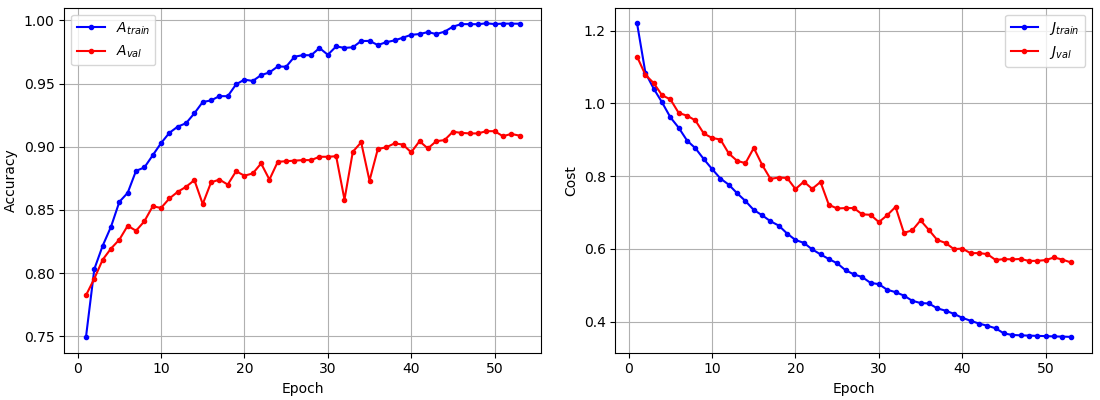
\includegraphics[width=1.0\textwidth]{figs/vgg16_total_convergence.png}
    \caption{Convergence of a transfer learning model where $e = f = 18$ and $\lambda = 0.00135721$.}
    \label{fig:vgg16_total_convergence}
\end{figure}

\begin{table}[ht]
\centering
\begin{tabular}{ |c|c|c|c|c| }
\hline
$e$ & $f$ & $\lambda$ & $A_{train}$ & $A_{val}$ \\
\hline
18 & 18 & 0.0001 & 1.0 & 0.914 \\
18 & 18 & 0.000154 & 0.995 & 0.9 \\
18 & 18 & 0.000239 & 1.0 & 0.911 \\
18 & 18 & 0.000368 & 1.0 & 0.908 \\
18 & 18 & 0.000569 & 0.994 & 0.904 \\
18 & 18 & 0.000879 & 0.998 & 0.911 \\
18 & 18 & 0.00136 & 0.998 & 0.911 \\
18 & 18 & 0.0021 & 0.994 & 0.908 \\
18 & 18 & 0.00324 & 0.991 & 0.902 \\
18 & 18 & 0.005 & 0.975 & 0.893 \\
\hline
 & & & $0.995\pm0.00713$ & $0.906\pm0.0061$ \\
\hline
\end{tabular}
\caption{Accuracy on the train set ($A_{train}$) and validation set ($A_{val}$) of transfer learning models where $e = 18$ and $f = 18$ are fixed and $\lambda$ is varied.}
\label{table:vgg16_total}
\end{table}

The validation curve of the L2-regularization strength $\lambda$ hyperparameter in figure \ref{fig:vgg16_total_lambda} shows these models are neither overfitting nor underfitting as $A_{val}$ is approximating $A_{train}$ well.

\begin{figure}[ht]
    \centering
    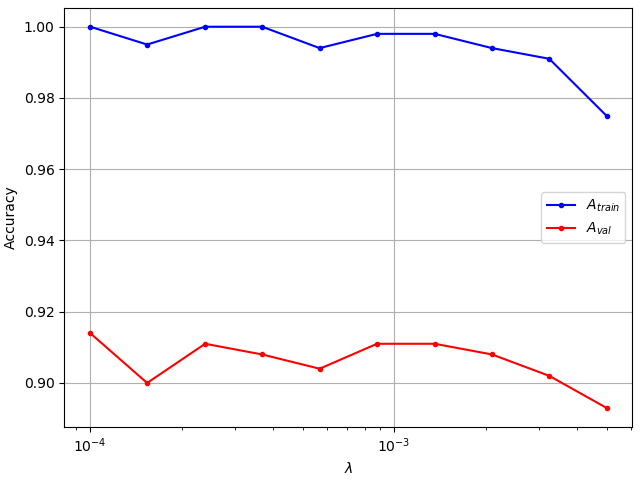
\includegraphics[width=1.0\textwidth]{figs/vgg16_total_lambda.png}
    \caption{Accuracy on the train set ($A_{train}$) and validation set ($A_{val}$) of transfer learning models where $e = 18$ and $f = 18$ are fixed and $\lambda$ is varied.}
    \label{fig:vgg16_total_lambda}
\end{figure}

Presumably these surprisingly good results stem from an appropriate number $m$ of training samples relative to the number of free parameters in the network as well as proper data augmentation. It is also important to remember that binary classification is a much easier optimization problem when compared to ImageNet's 1000-class classification task.

Indeed, by fixing $\lambda = 0.000879$ (for example) and varying the effective number of training samples as the first $m'$ of the original $m$ training samples it can be seen (in table \ref{table:vgg16_total_debug} and figure \ref{fig:vgg16_total_debug}) that performance increases as the number of samples increases. Therefore it is relatively safe to say the preprocessing steps described before suit the problem at hand.

\begin{table}[ht]
\centering
\begin{tabular}{ |c|c|c| }
\hline
$m'$ & $A_{train}$ & $A_{val}$ \\
\hline
1286 & 0.977 & 0.771  \\
2572 & 0.991 & 0.803  \\
3859 & 0.973 & 0.819  \\
5145 & 0.984 & 0.843  \\
6432 & 0.997 & 0.863  \\
7718 & 0.987 & 0.868  \\
9004 & 0.996 & 0.881  \\
10291 & 0.998 & 0.899 \\
11577 & 0.989 & 0.894 \\
\hline
 & $0.988\pm0.00829$ & $0.849\pm0.0412$ \\
\hline
\end{tabular}
\caption{Accuracy on the train set ($A_{train}$) and validation set ($A_{val}$) of transfer learning models when $e = 18$, $f = 18$, $\lambda = 0.000879$ are fixed and the number of train samples $m'$ is varied.}
\label{table:vgg16_total_debug}
\end{table}

\begin{figure}[ht]
    \centering
    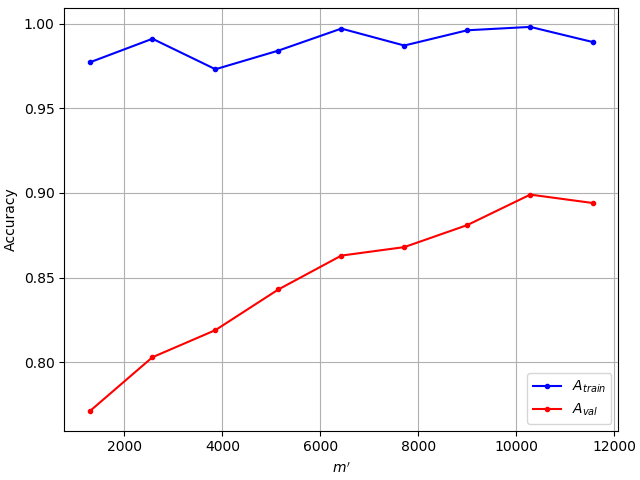
\includegraphics[width=1.0\textwidth]{figs/vgg16_total_debug.png}
    \caption{Accuracy on the train set ($A_{train}$) and validation set ($A_{val}$) of transfer learning models when $e = 18$, $f = 18$, $\lambda = 0.000879$ are fixed and the number of train samples $m'$ is varied.}
    \label{fig:vgg16_total_debug}
\end{figure}

\subsection{Partial Parameter Extraction}
\label{section:partial_parameter_extraction}

Extracting a smaller number $e < 18$ of layers is an interesting strategy since that would yield a smaller and faster model that could be used in applications with less computational resources. Besides, presumably, the most relevant features are likely being computed in the middle layers.

In this case, training specifically follows the methodology:

\begin{enumerate}
    \item Standardize training and validation samples relative to ImageNet;
    \item Define network architecture:
        \begin{enumerate}
            \item Extract $e < 18$ and freeze $f \leq e$ layers from the pre-trained model;
            \item Use global average pooling to reduce the number of parameters before the classifier based on fully-connected layers;
            \item Use one fully-connected layer of 512 ReLU-activated neurons;
            \item Use one fully-connected layer of 1 sigmoid-activated neuron for binary classification.
        \end{enumerate}
    \item Some parameters are transfered from pre-trained models and otherwise initialized according to Xavier initialization;
    \item Mini-batch \ac{SGD} with momentum $\gamma = 0.9$:
        \begin{itemize}
            \item Binary cross entropy cost function and explicit L2 regularization with cross-validated $\lambda \in [0.0001, 0.005]$ spaced evenly on a log scale;
            \item 32 samples batches;
            \item Initial learning rate $\eta = 10^{-4}$ that decays by a factor of $10$ if the validation accuracy has not improved $+10^{-3}$ in the last $10$ epochs;
            \item Shuffle the $m$ samples every epoch;
            \item Train for a maximum of 1000 epochs, stopping early if the loss has not changed $\pm 10^{-3}$ in the last $30$ epochs.
        \end{itemize}
\end{enumerate}

However none of the models converge usefully, likely stuck in a local minimum with high loss (e.g., figure \ref{fig:vgg16_partial_divergence}).

\begin{figure}[ht]
    \centering
    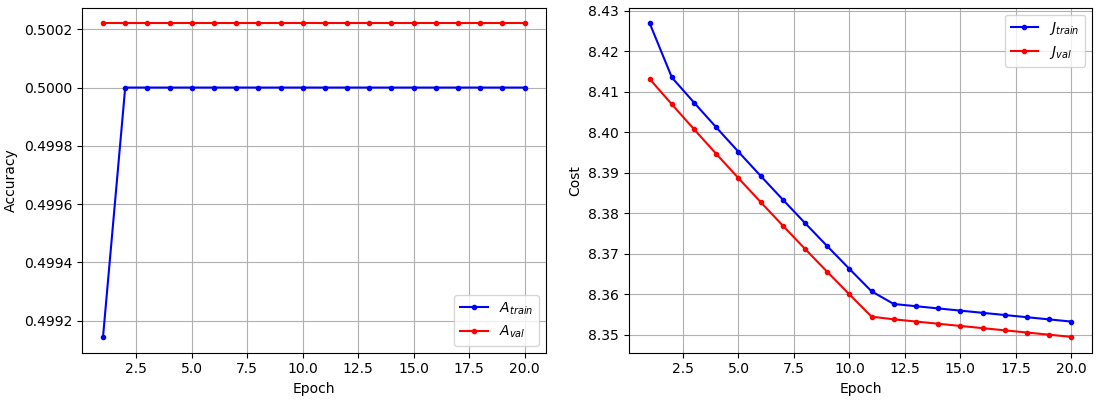
\includegraphics[width=1.0\textwidth]{figs/vgg16_partial_divergence.png}
    \caption{Partial parameter extraction model (with $e = 14$, $f = 14$, $\lambda = 0.00015445$, $\eta = 10^{-4}$) not converging, stuck in a local minimum.}
    \label{fig:vgg16_partial_divergence}
\end{figure}

Accordingly, performance results (in table \ref{table:vgg16_partial}) are disappointing for any number $e < 18$ of frozen layers (for brevity only $e = 10$ is presented in table \ref{table:vgg16_partial}).

\begin{table}[ht]
\centering
\begin{tabular}{ |c|c|c|c|c| }
\hline
$e$ & $f$ & $\lambda$ & $A_{train}$ & $A_{val}$ \\
\hline
10 & 0 & 0.0001 & 0.5 & 0.5 \\
10 & 0 & 0.000154 & 0.5 & 0.5 \\
10 & 0 & 0.000239 & 0.5 & 0.5 \\
10 & 0 & 0.000368 & 0.5 & 0.5 \\
10 & 0 & 0.000569 & 0.5 & 0.5 \\
10 & 0 & 0.000879 & 0.5 & 0.5 \\
10 & 0 & 0.00136 & 0.5 & 0.5 \\
10 & 0 & 0.0021 & 0.5 & 0.5 \\
10 & 0 & 0.00324 & 0.5 & 0.5 \\
10 & 0 & 0.005 & 0.5 & 0.5 \\
10 & 3 & 0.0001 & 0.5 & 0.5 \\
10 & 3 & 0.000154 & 0.5 & 0.5 \\
10 & 3 & 0.000239 & 0.5 & 0.5 \\
10 & 3 & 0.000368 & 0.5 & 0.5 \\
10 & 3 & 0.000569 & 0.5 & 0.5 \\
10 & 3 & 0.000879 & 0.5 & 0.5 \\
10 & 3 & 0.00136 & 0.5 & 0.5 \\
10 & 3 & 0.0021 & 0.5 & 0.5 \\
10 & 3 & 0.00324 & 0.5 & 0.5 \\
10 & 3 & 0.005 & 0.5 & 0.5 \\
10 & 6 & 0.0001 & 0.5 & 0.5 \\
10 & 6 & 0.000154 & 0.5 & 0.5 \\
10 & 6 & 0.000239 & 0.5 & 0.5 \\
10 & 6 & 0.000368 & 0.5 & 0.5 \\
10 & 6 & 0.000569 & 0.5 & 0.5 \\
10 & 6 & 0.000879 & 0.5 & 0.5 \\
10 & 6 & 0.00136 & 0.5 & 0.5 \\
10 & 6 & 0.0021 & 0.5 & 0.5 \\
10 & 6 & 0.00324 & 0.5 & 0.5 \\
10 & 6 & 0.005 & 0.5 & 0.5 \\
10 & 10 & 0.0001 & 0.5 & 0.5 \\
10 & 10 & 0.000154 & 0.5 & 0.5 \\
10 & 10 & 0.000239 & 0.5 & 0.5 \\
10 & 10 & 0.000368 & 0.5 & 0.5 \\
10 & 10 & 0.000569 & 0.5 & 0.5 \\
10 & 10 & 0.000879 & 0.5 & 0.5 \\
10 & 10 & 0.00136 & 0.5 & 0.5 \\
10 & 10 & 0.0021 & 0.5 & 0.5 \\
10 & 10 & 0.00324 & 0.5 & 0.5 \\
10 & 10 & 0.005 & 0.5 & 0.5 \\
\hline
 & & & $0.5\pm0.0$ & $0.5\pm0.0$ \\
\hline
\end{tabular}
    \caption{Accuracy on the train set ($A_{train}$) and validation set ($A_{val}$) of transfer learning models where $e$ (for brevity only $e = 10$ is shown), $f$, and $\lambda$ are varied.}
\label{table:vgg16_partial}
\end{table}

To explain this, it was hypothesized that the learning rate $\eta = 10^{-4}$ was adequate for the higher layers of the fifth convolutional block, but too high for the remaining layers where \ac{SGD} was overshooting the update of the parameters. Intuitively, the high learning rate was disrupting the parameters learned by the pre-trained model.

Fixing $e = 14$, $f = 14$, $\lambda = 0.00015445$ (for example) and cross-validating 20 new smaller values for the learning rate (from $\eta \in [10^0, 10^{-10}]$ spaced evenly on a log-scale) yields converging models with very good performance (figure \ref{fig:vgg16_partial_lr}), which confirms the hypothesis.

\begin{figure}[ht]
    \centering
    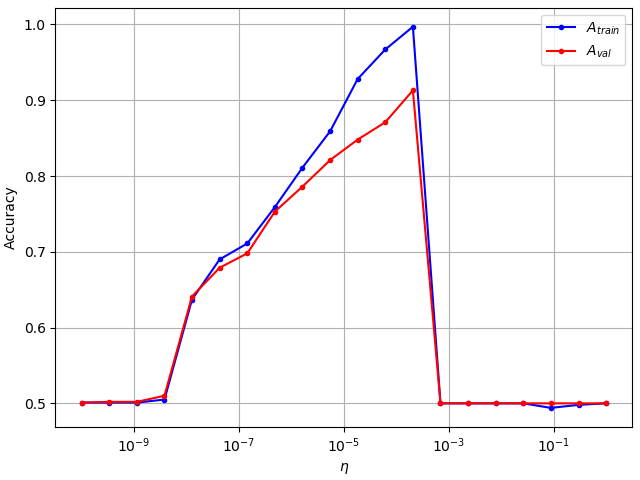
\includegraphics[width=1.0\textwidth]{figs/vgg16_partial_lr.png}
    \caption{Accuracy on the train set ($A_{train}$) and validation set ($A_{val}$) of transfer learning models where $e = 14$, $f = 14$, $\lambda = 0.00015445$ are fixed and $\eta$ is varied.}
    \label{fig:vgg16_partial_lr}
\end{figure}

For example, $\eta = 0.000206913808$ was found to provide convergence (figure \ref{fig:vgg16_partial_convergence}) to accuracy on the validation set $A_{val} = 0.913$ while only extracting $e = 14$ layers which makes for a smaller, faster model.

\begin{figure}[ht]
    \centering
    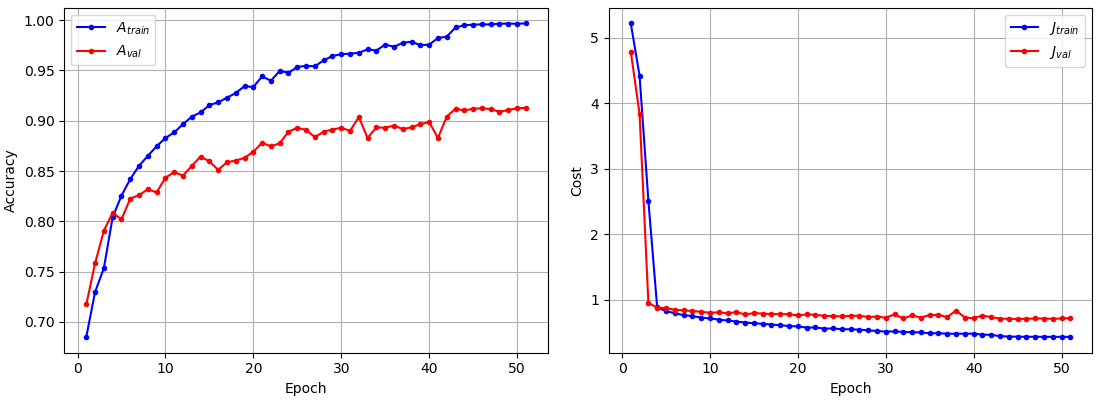
\includegraphics[width=1.0\textwidth]{figs/vgg16_partial_convergence.png}
    \caption{Partial parameter extraction model (with $e = 14$, $f = 14$, $\lambda = 0.00015445$, $\eta = 10^{-4}$) converging to very good performance while maintaining modest model size.}
    \label{fig:vgg16_partial_convergence}
\end{figure}

A more thorough systematic study of the learning rate (or different optimizers) when extracting lower-level layers would certainly unveil more models with a good balance between model size and model performance, perhaps even outperforming models that extract all layers.

\subsection{Total Parameter Extraction with Fine Tuning}
\label{section:total_parameter_extraction_with_fine_tuning}

Extracting all layers ($e = 18$) while also fine-tuning these layers ($f \leq e$) will presumably yield higher performance since it will continue to optimize parameters relative to the target dataset, thus minimizing error on said dataset and generalizing well to similar test data.

In this case, training specifically follows the methodology:

\begin{enumerate}
    \item Standardize training and validation samples relative to ImageNet;
    \item Define network architecture:
        \begin{enumerate}
            \item Extract $e = 18$ and freeze $f \leq e$ layers from the pre-trained model;
            \item Use global average pooling to reduce the number of parameters before the classifier based on fully-connected layers;
            \item Use one fully-connected layer of 512 ReLU-activated neurons;
            \item Use one fully-connected layer of 1 sigmoid-activated neuron for binary classification.
        \end{enumerate}
    \item Some parameters are transfered from pre-trained models and otherwise initialized according to Xavier initialization;
    \item Mini-batch \ac{SGD} with momentum $\gamma = 0.9$:
        \begin{itemize}
            \item Binary cross entropy cost function and explicit L2 regularization with cross-validated $\lambda \in [0.0001, 0.005]$ spaced evenly on a log scale;
            \item 32 samples batches;
            \item Initial learning rate $\eta = 10^{-4}$ that decays by a factor of $10$ if the validation accuracy has not improved $+10^{-3}$ in the last $10$ epochs;
            \item Shuffle the $m$ samples every epoch;
            \item Train for a maximum of 1000 epochs, stopping early if the loss has not changed $\pm 10^{-3}$ in the last $30$ epochs.
        \end{itemize}
\end{enumerate}

Indeed, freezing the first $f = 14$ layers yields, on average, an 8\% increase (relative to the previous $e = f = 18$ configurations in table \ref{table:vgg16_total}) in accuracy on the validation set (table \ref{table:vgg16_finetuning_14}).

\begin{table}[ht]
\centering
\begin{tabular}{ |c|c|c|c|c| }
\hline
$e$ & $f$ & $\lambda$ & $A_{train}$ & $A_{val}$ \\
\hline
18 & 14 & 0.0001 & 1.0 & 0.928 \\
18 & 14 & 0.000154 & 1.0 & 0.923 \\
18 & 14 & 0.000239 & 1.0 & 0.925 \\
18 & 14 & 0.000368 & 1.0 & 0.926 \\
18 & 14 & 0.000569 & 1.0 & 0.925 \\
18 & 14 & 0.000879 & 1.0 & 0.921 \\
18 & 14 & 0.00136 & 1.0 & 0.923 \\
18 & 14 & 0.0021 & 1.0 & 0.927 \\
18 & 14 & 0.00324 & 1.0 & 0.925 \\
18 & 14 & 0.005 & 1.0 & 0.925 \\
\hline
 & & & $1.0\pm0.0$ & $0.925\pm0.00194$ \\
\hline
\end{tabular}
\caption{Accuracy on the train set ($A_{train}$) and validation set ($A_{val}$) of transfer learning models when $e = 18$ and $f = 14$ are fixed and $\lambda$ is varied.}
\label{table:vgg16_finetuning_14}
\end{table}

However, as more layers are unfrozen (i.e., $f$ takes smaller values) some models do not converge for specific values of $\lambda$:

\begin{itemize}
    \item when $f = 10$ one of the ten models does not converge (table \ref{table:vgg16_finetuning_10});

    \begin{table}[ht]
    \centering
    \begin{tabular}{ |c|c|c|c|c| }
    \hline
    $e$ & $f$ & $\lambda$ & $A_{train}$ & $A_{val}$ \\
    \hline
    18 & 10 & 0.0001 & 0.5 & 0.5 \\
    18 & 10 & 0.000154 & 1.0 & 0.926 \\
    18 & 10 & 0.000239 & 1.0 & 0.928 \\
    18 & 10 & 0.000368 & 1.0 & 0.922 \\
    18 & 10 & 0.000569 & 1.0 & 0.933 \\
    18 & 10 & 0.000879 & 1.0 & 0.925 \\
    18 & 10 & 0.00136 & 1.0 & 0.935 \\
    18 & 10 & 0.0021 & 1.0 & 0.931 \\
    18 & 10 & 0.00324 & 1.0 & 0.929 \\
    18 & 10 & 0.005 & 1.0 & 0.929 \\
    \hline
     & & & $0.95\pm0.15$ & $0.886\pm0.129$ \\
    \hline
    \end{tabular}
    \caption{Accuracy on the train set ($A_{train}$) and validation set ($A_{val}$) of transfer learning models when $e = 18$ and $f = 10$ are fixed and $\lambda$ is varied.}
    \label{table:vgg16_finetuning_10}
    \end{table}

    \item when $f = 6$ five of the ten models do not converge (table \ref{table:vgg16_finetuning_6});

    \begin{table}[ht]
    \centering
    \begin{tabular}{ |c|c|c|c|c| }
    \hline
    $e$ & $f$ & $\lambda$ & $A_{train}$ & $A_{val}$ \\
    \hline
    18 & 6 & 0.0001 & 0.5 & 0.5 \\
    18 & 6 & 0.000154 & 0.5 & 0.5 \\
    18 & 6 & 0.000239 & 1.0 & 0.93 \\
    18 & 6 & 0.000368 & 0.5 & 0.5 \\
    18 & 6 & 0.000569 & 1.0 & 0.925 \\
    18 & 6 & 0.000879 & 1.0 & 0.922 \\
    18 & 6 & 0.00136 & 0.5 & 0.501 \\
    18 & 6 & 0.0021 & 0.501 & 0.498 \\
    18 & 6 & 0.00324 & 1.0 & 0.917 \\
    18 & 6 & 0.005 & 1.0 & 0.922 \\
    \hline
     & & & $0.75\pm0.25$ & $0.711\pm0.212$ \\
    \hline
    \end{tabular}
    \caption{Accuracy on the train set ($A_{train}$) and validation set ($A_{val}$) of transfer learning models when $e = 18$ and $f = 6$ are fixed and $\lambda$ is varied.}
    \label{table:vgg16_finetuning_6}
    \end{table}

    \item when $f = 3$ four of the ten models do not converge (table \ref{table:vgg16_finetuning_3});

    \begin{table}[ht]
    \centering
    \begin{tabular}{ |c|c|c|c|c| }
    \hline
    $e$ & $f$ & $\lambda$ & $A_{train}$ & $A_{val}$ \\
    \hline
    18 & 3 & 0.0001 & 1.0 & 0.9 \\
    18 & 3 & 0.000154 & 0.5 & 0.5 \\
    18 & 3 & 0.000239 & 0.5 & 0.5 \\
    18 & 3 & 0.000368 & 1.0 & 0.915 \\
    18 & 3 & 0.000569 & 1.0 & 0.926 \\
    18 & 3 & 0.000879 & 1.0 & 0.927 \\
    18 & 3 & 0.00136 & 1.0 & 0.933 \\
    18 & 3 & 0.0021 & 1.0 & 0.931 \\
    18 & 3 & 0.00324 & 0.5 & 0.5 \\
    18 & 3 & 0.005 & 0.5 & 0.5 \\
    \hline
     & & & $0.8\pm0.245$ & $0.753\pm0.207$ \\
    \hline
    \end{tabular}
    \caption{Accuracy on the train set ($A_{train}$) and validation set ($A_{val}$) of transfer learning models when $e = 18$ and $f = 3$ are fixed and $\lambda$ is varied.}
    \label{table:vgg16_finetuning_3}
    \end{table}

    \item when $f = 0$ eight of the ten models do not converge (table \ref{table:vgg16_finetuning_0}).

    \begin{table}[ht]
    \centering
    \begin{tabular}{ |c|c|c|c|c| }
    \hline
    $e$ & $f$ & $\lambda$ & $A_{train}$ & $A_{val}$ \\
    \hline
    18 & 0 & 0.0001 & 0.5 & 0.5 \\
    18 & 0 & 0.000154 & 1.0 & 0.916 \\
    18 & 0 & 0.000239 & 1.0 & 0.9 \\
    18 & 0 & 0.000368 & 0.5 & 0.5 \\
    18 & 0 & 0.000569 & 0.5 & 0.5 \\
    18 & 0 & 0.000879 & 0.501 & 0.5 \\
    18 & 0 & 0.00136 & 0.5 & 0.5 \\
    18 & 0 & 0.0021 & 0.5 & 0.5 \\
    18 & 0 & 0.00324 & 0.5 & 0.5 \\
    18 & 0 & 0.005 & 0.5 & 0.5 \\
    \hline
     & & & $0.6\pm0.2$ & $0.582\pm0.163$ \\
    \hline
    \end{tabular}
    \caption{Accuracy on the train set ($A_{train}$) and validation set ($A_{val}$) of transfer learning models when $e = 18$ and $f = 0$ are fixed and $\lambda$ is varied.}
    \label{table:vgg16_finetuning_0}
    \end{table}

\end{itemize}

In other words, as more layers are unfrozen, a progressively bigger number of models does not converge, but for each setting of $e$ and $f$ there is always a converging model which indicates some sensitivity to the regularization parameter $\lambda$.

This can be explained by an inadequate setting of the learning rate just as in the previous set of experiments. The more higher layers are unfrozen, the more their weights are disrupted too quickly because of too high a learning rate. Cross-validating a range of smaller learning rates (perhaps carefully chosen on a per-layer basis) would certainly unveil models with good performance, as seen before. However it is also possible that using the Adam optimizer could unveil models with good performance, since it maintains a distinct and adaptive learning rate per parameter in the network.

By fixing $e = 18$, $f = 0$, $\lambda = 0.0003684$ a new model was trained identically but using the Adam optimizer instead, with an initial learning rate $\eta = 10^{-8}$ and hyperparameters $\beta_1=0.9$, $\beta_2=0.999$, and $\epsilon=1e-{7}$. Unlike similar models trained with \ac{SGD}, this model converged very smoothly (figure \ref{fig:vgg16_adam}) to an accuracy on the validation set of $A_{val} = 0.836$.

\begin{figure}[ht]
    \centering
    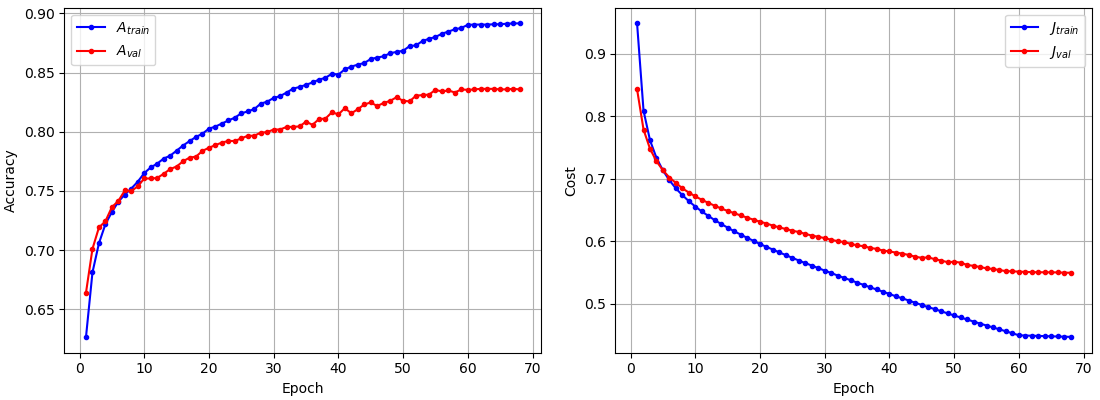
\includegraphics[width=1.0\textwidth]{figs/vgg16_adam.png}
    \caption{Convergence of a transfer learning model (with $e = 18$ and $f = 0$) trained with the Adam optimizer with an initial learning rate $\eta = 10^{-8}$ which would otherwise not converge.}
    \label{fig:vgg16_adam}
\end{figure}

\section{End-to-End Learning Experiments}
\label{section:endtoend}

This section describes a set of experiments involving models of custom designed \ac{CNN} architectures trained from scratch, following the more traditional methodology typically called end-to-end learning, that will be used for comparison against the transfer learning approach which it is in direct contrast with.

Designing a custom \ac{CNN} architecture from scratch is quite difficult as it requires setting and reasoning about many different hyperparameters simultaneously (number of convolutional layers, number of filters in each layer, size of filters, stride, etc.) for which there is no one right answer; hyperparameters should always be cross-validated from a wide range on the problem at hand. Instead, these custom architectures will be based around reasonable heuristics \cite{cs231n} extrapolated from the training of successful deep networks:

\begin{itemize}
    \item The most common architecture of convolutional neural networks is to stack ReLU-activated convolutional layers followed by a max pooling layer, a pattern which is arbitrarily repeated to some desired depth in order to reduce the dimensions of the features, after which it is common to use fully-connected layers;
    \item Prefer a stack of many small filters in convolutional layers rather than one large filter;
    \item Use zero-padding and stride $S = 1$ in convolutional layers as they provide better performance;
    \item Prefer $2 \times 2$ filters with stride $S = 2$ in pooling layers to avoid aggressive, lossy downsampling and consequently worse performance.
\end{itemize}

\subsection{Custom Architecture 1}

This custom architecture, illustrated in figure \ref{fig:custom1}, stacks three convolution-pooling blocks. Each block stacks two convolutional layers before the pooling layer, which is a good idea for large and deep networks because multiple stacked convolutional layers can develop more complex features of the input volume before the destructive pooling operation. Specifically,

\begin{enumerate}
    \item 32 $3 \times 3$ filters, stride of 1, zero padding, ReLU activated
    \item 32 $3 \times 3$ filters, stride of 1, zero padding, ReLU activated
    \item $2 \times 2$ max pooling with stride 2
    \item 64 $3 \times 3$ filters, stride of 1, zero padding, ReLU activated
    \item 64 $3 \times 3$ filters, stride of 1, zero padding, ReLU activated
    \item $2 \times 2$ max pooling with stride 2
    \item 128 $3 \times 3$ filters, stride of 1, zero padding, ReLU activated
    \item 128 $3 \times 3$ filters, stride of 1, zero padding, ReLU activated
\end{enumerate}

The classifier, illustrated in figure \ref{fig:custom1}, is a stack of two fully-connected layers of ReLU-activated neurons followed by a fully-connected sigmoid-activated neuron for binary classification.

\begin{enumerate}
    \item 512 fully-connected ReLU-activated neurons;
    \item Another 512 fully-connected ReLU-activated neurons;
    \item Single fully-connected sigmoid-activated neuron for binary classification.
\end{enumerate}

\begin{figure}[ht]
    \centering
    \includegraphics[width=1.0\textwidth]{figs/custom1.png}
    \caption{Custom \ac{CNN} architecture 1.}
    \label{fig:custom1}
\end{figure}

Models of this architecture are trained identically as follows:

\begin{enumerate}
    \item Standardize training and validation samples relative to \ac{ISIC} 2018;
    \item Define network architecture:
        \begin{enumerate}
            \item Stack three blocks of convolutional and pooling layers to build useful features for classification;
            \item Use global average pooling to reduce the number of parameters before the classifier based on fully-connected layers;
            \item Stack two fully-connected layers of 512 ReLU-activated neurons;
            \item Use fully-connected layer with a single sigmoid-activated neuron for binary classification.
        \end{enumerate}
    \item Parameters are all initialized according to Xavier initialization;
    \item Mini-batch \ac{SGD} with momentum $\gamma = 0.9$:
        \begin{itemize}
            \item Binary cross entropy cost function and explicit L2 regularization with cross-validated $\lambda \in [0.0001, 0.005]$ spaced evenly on a log scale;
            \item 32 samples batches;
            \item Shuffle the $m$ samples every epoch;
            \item Initial learning rate $\eta = 10^{-4}$ that decays by a factor of $10$ if the validation accuracy has not improved $+10^{-3}$ in the last $10$ epochs;
            \item Train for a maximum of 1000 epochs, stopping early if the loss has not changed $\pm 10^{-3}$ in the last $30$ epochs.
        \end{itemize}
\end{enumerate}

The results of this set of experiments are summarized in table \ref{table:custom1_all}.

\begin{table}[ht]
\centering
\begin{tabular}{ |c|c|c|c|c|c|c|c| }
\hline
$\lambda$ & $A_{train}$ & $A_{val}$ \\
\hline
0.0001 & 0.737 & 0.726 \\
0.000154 & 0.734 & 0.724 \\
0.000239 & 0.795 & 0.785 \\
0.000368 & 0.782 & 0.768 \\
0.000569 & 0.723 & 0.72 \\
0.000879 & 0.724 & 0.72 \\
0.00136 & 0.723 & 0.718 \\
0.0021 & 0.721 & 0.716 \\
0.00324 & 0.719 & 0.709 \\
0.005 & 0.713 & 0.704 \\
\hline
 & $0.737\pm0.0267$ & $0.729\pm0.0248$ \\
\hline
\end{tabular}
\caption{Performance metrics of models of the custom architecture 1 where $\lambda$ is varied.}
\label{table:custom1_all}
\end{table}

The effect of $\lambda$ on the performance of the model can be understood in figure \ref{fig:custom1_lambda}.

\begin{figure}[ht]
    \centering
    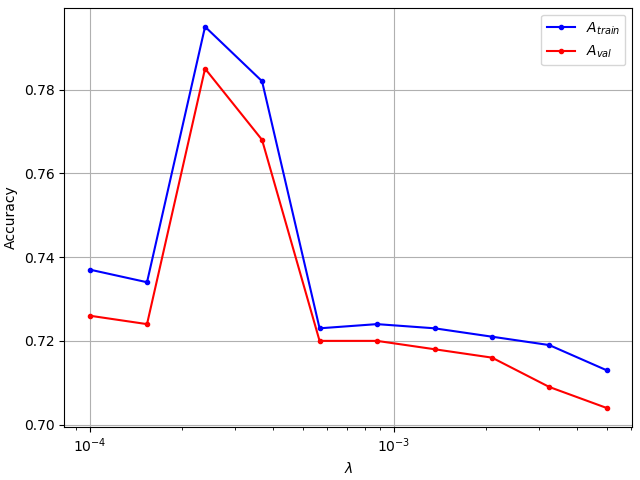
\includegraphics[width=1.0\textwidth]{figs/custom1_lambda.png}
    \caption{Accuracy on the train set ($A_{train}$) and validation set ($A_{val}$) of models of the custom architecture 1 over a range of values for L2-regularization strength $\lambda$.}
    \label{fig:custom1_lambda}
\end{figure}

In particular, $\lambda = 0.000239$ gives the best performing model of the custom architecture 1 ($A_{val} = 0.785$). The convergence of this model can be tracked in figure \ref{fig:custom1_best_training}.

\begin{figure}[ht]
    \centering
    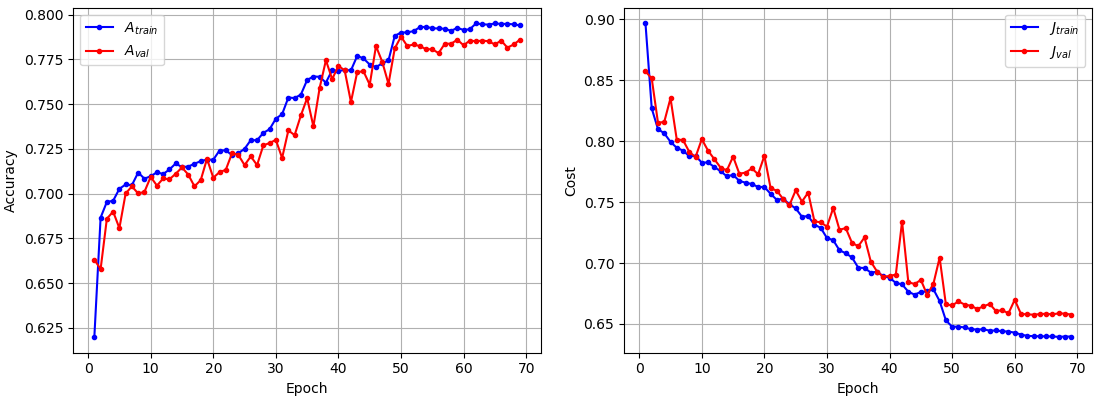
\includegraphics[width=1.0\textwidth]{figs/custom1_best_training.png}
    \caption{Convergence of the best model of the custom architecture 1.}
    \label{fig:custom1_best_training}
\end{figure}

\subsection{Custom Architecture 2}

This custom architecture, illustrated in figure \ref{fig:custom2}, stacks two convolution-pooling blocks. Each block uses a single convolutional layer before the pooling layer:

\begin{enumerate}
    \item 32 $3 \times 3$ filters, stride of 1, zero padding, ReLU activated;
    \item $2 \times 2$ max pooling with stride of 2;
    \item 64 $3 \times 3$ filters, stride of 1, zero padding, ReLU activated;
    \item $2 \times 2$ max pooling with stride of 2.
\end{enumerate}

The classifier is a single fully-connected layer of 512 ReLU-activated neurons followed by a fully-connected sigmoid-activated neuron for binary classification:

\begin{enumerate}
    \item 512 fully-connected ReLU-activated neurons;
    \item Single fully-connected sigmoid-activated neuron for binary classification.
\end{enumerate}

\begin{figure}[ht]
    \centering
    \includegraphics[width=1.0\textwidth]{figs/custom2.png}
    \caption{Custom \ac{CNN} architecture 2.}
    \label{fig:custom2}
\end{figure}

Models of this architecture are trained identically as follows:

\begin{enumerate}
    \item Standardize training and validation samples relative to \ac{ISIC} 2018;
    \item Define network architecture:
        \begin{enumerate}
            \item Stack two blocks of convolutional and pooling layers to build useful features for classification;
            \item Use global average pooling to reduce the number of parameters before the classifier based on fully-connected layers;
            \item Use fully-connected layers of 512 ReLU-activated neurons;
            \item Use fully-connected layer with a single sigmoid-activated neuron for binary classification.
        \end{enumerate}
    \item Parameters are all initialized according to Xavier initialization;
    \item Mini-batch \ac{SGD} with momentum $\gamma = 0.9$:
        \begin{itemize}
            \item Binary cross entropy cost function and explicit L2 regularization with cross-validated $\lambda \in [0.0001, 0.005]$ spaced evenly on a log scale;
            \item 32 samples batches;
            \item Shuffle the $m$ samples every epoch;
            \item Initial learning rate $\eta = 10^{-4}$ that decays by a factor of $10$ if the validation accuracy has not improved $+10^{-3}$ in the last $10$ epochs;
            \item Train for a maximum of 1000 epochs, stopping early if the loss has not changed $\pm 10^{-3}$ in the last $30$ epochs.
        \end{itemize}
\end{enumerate}

The results of this set of experiments are summarized in table \ref{table:custom2_all}.

\begin{table}[ht]
\centering
\begin{tabular}{ |c|c|c|c|c|c|c|c| }
\hline
$\lambda$ & $A_{train}$ & $A_{val}$ \\
\hline
0.0001 & 0.737 & 0.724 \\
0.000154 & 0.736 & 0.72 \\
0.000239 & 0.734 & 0.72 \\
0.000368 & 0.731 & 0.717 \\
0.000569 & 0.724 & 0.716 \\
0.000879 & 0.724 & 0.719 \\
0.00136 & 0.725 & 0.719 \\
0.0021 & 0.718 & 0.71 \\
0.00324 & 0.714 & 0.706 \\
0.005 & 0.711 & 0.703 \\
\hline
 & $0.725\pm0.00865$ & $0.715\pm0.00645$ \\
\hline
\end{tabular}
\caption{Performance metrics of models of the custom architecture 2 where $\lambda$ is varied.}
\label{table:custom2_all}
\end{table}

The effect of $\lambda$ on the performance of the model can be understood in figure \ref{fig:custom2_lambda}.

\begin{figure}[ht]
    \centering
    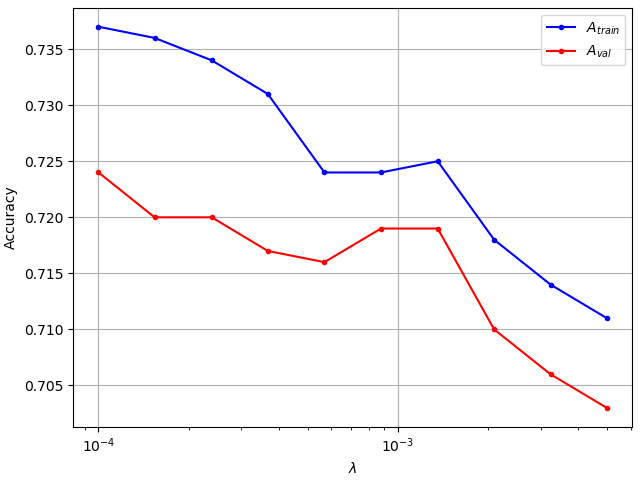
\includegraphics[width=1.0\textwidth]{figs/custom2_lambda.png}
    \caption{Accuracy on the train set ($A_{train}$) and validation set ($A_{val}$) of models of the custom architecture 2 over a range of values for L2-regularization strength $\lambda$.}
    \label{fig:custom2_lambda}
\end{figure}

In particular, $\lambda = 0.0001$ gives the best performing model of the custom architecture 2 ($A_{val} = 0.724$). The convergence of this model can be tracked in figure \ref{fig:custom2_best_training}.

\begin{figure}[ht]
    \centering
    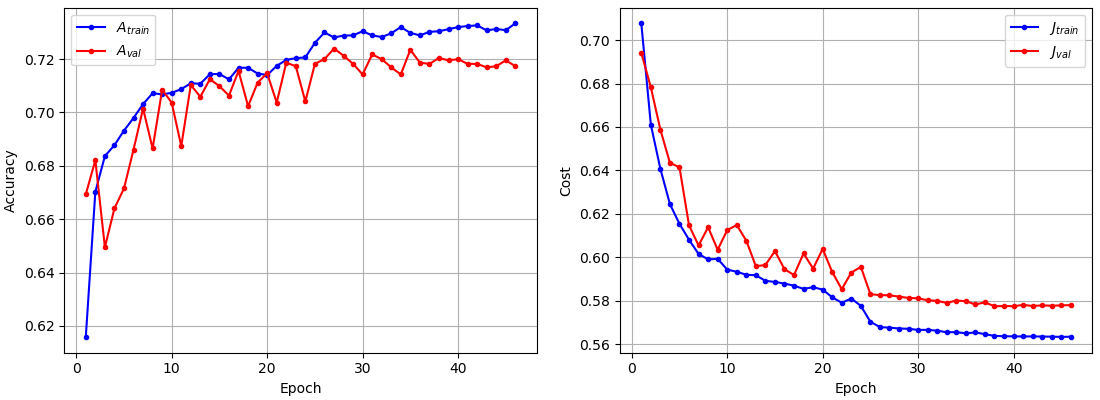
\includegraphics[width=1.0\textwidth]{figs/custom2_best_training.png}
    \caption{Convergence of the best model of the custom architecture 2.}
    \label{fig:custom2_best_training}
\end{figure}

\section{Discussion}

Sufficient labeled data is hard to come by in a lot of problems and it greatly impacts generalization performance. That is one void that transfer learning tries to fill but, in addition to such learning techniques, it is crucial to simultaneously fix the problem at the source and perform data augmentation to squeeze as much new quality data as possible (as seen in section \ref{section:total_parameter_extraction_without_fine_tuning} where parameters are extracted at the highest layer without retraining).

From the experiments in section \ref{section:partial_parameter_extraction} where parameters are extracted from lower layers it was seen that the learning rate plays an important role in transfer learning, since different layers in pre-trained models appear to respond differently to the learning rate and \ac{SGD} overshoots the update in gradient descent, effectively disrupting the learned features. Similarly, the experiments in section \ref{section:total_parameter_extraction_with_fine_tuning} (where parameters are extracted at the highest layer, but retrained) show that an adaptive optimizer like Adam can solve the same fundamental issue, i.e., updating parameters of lower layers at an inappropriate learning rate.

Lastly, in section \ref{section:endtoend} it was shown that end-to-end learning is much more difficult given the number of different hyperparameters that need to be reasoned about and set accordingly in cross-validation, which for most problems and most research teams is just too computationally intensive.

The best models are evaluated and compared primarily using accuracy as measured on the test set $A_{test}$, as well as $AUC$, precison $P$, recall $R$, and F1-score $F_1$ for comparison (table \ref{table:comparison}). It is worth noting how the train set was evidently class-balanced correctly since $F_1 \approx A_{test}$.

\begin{table}[ht]
\centering
\begin{tabular}{ |c|c|c|c|c|c| }
\hline
Model & $A_{test}$ & $AUC$ & $P$ & $R$ & $F_1$ \\
\hline
Custom 2 $\lambda = 0.0003684$                   & 0.738 & 0.737 & 0.761 & 0.738 & 0.732 \\
Custom 1 $\lambda = 0.00023853$                  & 0.781 & 0.781 & 0.785 & 0.781 & 0.78  \\
VGG16 $e = 18$, $f = 10$, $\lambda = 0.00056898$ & 0.943 & 0.943 & 0.945 & 0.943 & 0.943 \\
\hline
\end{tabular}
\caption{Comparison of metrics on the test set of the best models.}
\label{table:comparison}
\end{table}

Overlapping the accuracies on the test set for the same values of $\lambda$ shows (in figure \ref{fig:comparison}) that transfer learning is a very practical solution, outperforming all other models regardless of the specific value of $\lambda$ (except for the one case where training did not converge because of inappropriate learning rate $\eta$ as was discussed).

\begin{figure}[ht]
    \centering
    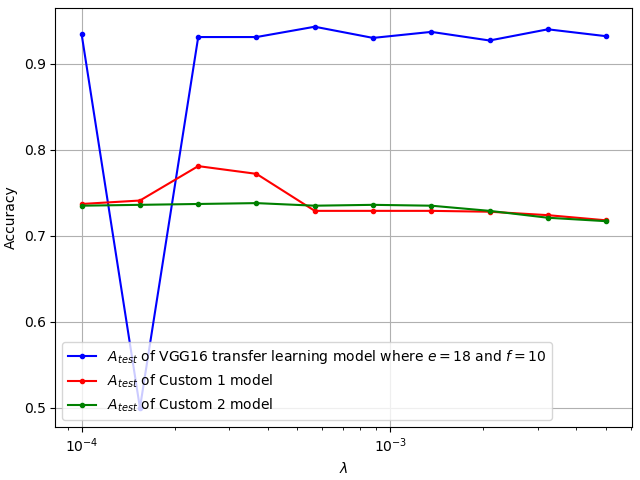
\includegraphics[width=1.0\textwidth]{figs/comparison.png}
    \caption{Overlapping accuracies on the test set of the best models.}
    \label{fig:comparison}
\end{figure}

The confusion matrix

\begin{itemize}
    \item of the best VGG16 transfer learning model is in figure \ref{fig:vgg16_best_confusionmatrix};
    \item of the best custom 1 model is in figure \ref{fig:custom1_best_confusionmatrix};
    \item of the best custom 2 model is in figure \ref{fig:custom2_best_confusionmatrix}.
\end{itemize}

\begin{figure}[ht]
    \centering
    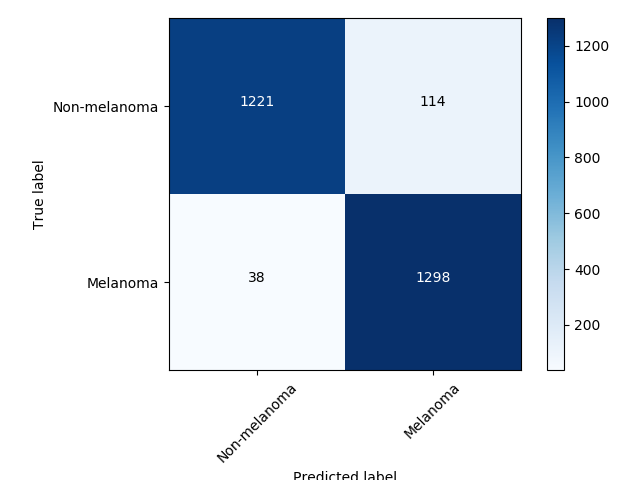
\includegraphics[width=1.0\textwidth]{figs/vgg16_best_confusionmatrix.png}
    \caption{Confusion matrix of the best VGG16 transfer learning model.}
    \label{fig:vgg16_best_confusionmatrix}
\end{figure}

\begin{figure}[ht]
    \centering
    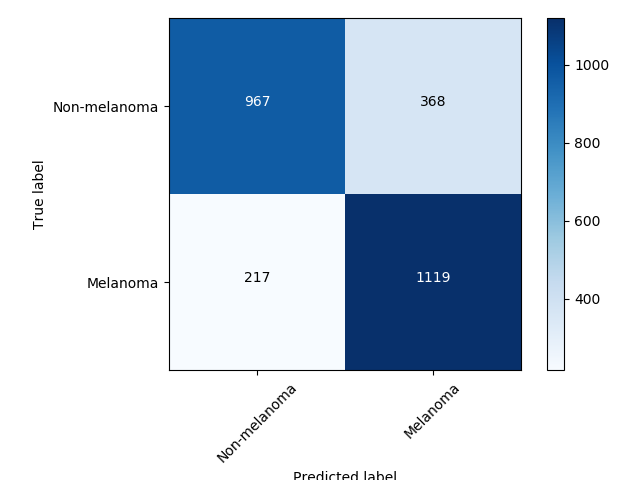
\includegraphics[width=1.0\textwidth]{figs/custom1_best_confusionmatrix.png}
    \caption{Confusion matrix of the best model of the custom architecture 1.}
    \label{fig:custom1_best_confusionmatrix}
\end{figure}

\begin{figure}[ht]
    \centering
    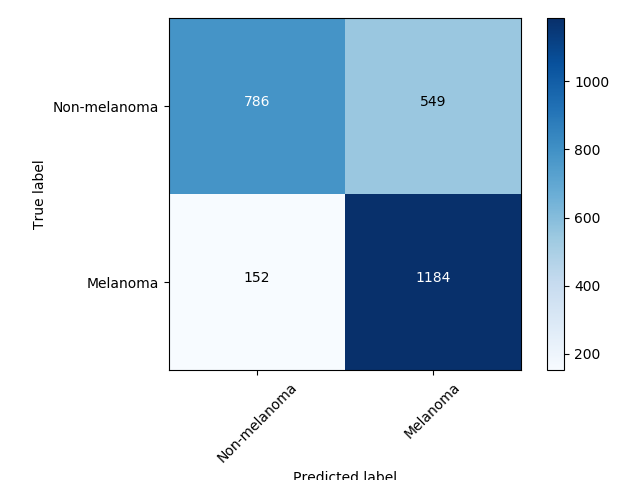
\includegraphics[width=1.0\textwidth]{figs/custom2_best_confusionmatrix.png}
    \caption{Confusion matrix of the best model of the custom architecture 2.}
    \label{fig:custom2_best_confusionmatrix}
\end{figure}
